\documentclass[11pt]{article}
\usepackage[toc,page]{appendix}
\usepackage{amsmath, amssymb}
\usepackage[utf8]{inputenc}
\usepackage[T1]{fontenc}
\usepackage[style=apa,backend=biber]{biblatex}
%\usepackage{biblatex}
\addbibresource{references.bib}
\usepackage{graphicx}
\usepackage{tikz}
\usetikzlibrary{automata,positioning,shapes.geometric, arrows.meta, fit, backgrounds, calc, chains}
\graphicspath{./images/Easy_Pictures/SMR_MULT_Repackaging}%\usepackage{kpfonts}
\usepackage{float}
\usepackage[margin=1in]{geometry}
\usepackage{cancel}
\usepackage{epsfig}
\usepackage{tikz-3dplot}
\usepackage{darkmode}
\usepackage{dirtytalk}
\usepackage{longtable,booktabs,array}
\usepackage{calc} % for calculating minipage widths
\usepackage[utf8]{inputenc}
\usepackage[T1]{fontenc}
\usepackage{xcolor}
\usepackage{listings}


\usepackage{etoolbox}
\usepackage{hyperref}
\hypersetup{
    colorlinks=true,
    linkcolor=blue,
    filecolor=magenta,      
    urlcolor=cyan,
    pdftitle={Hermeneutic Calculator},
    citecolor=blue,
    }


\urlstyle{same}

\lstdefinestyle{htmlStyle}{
    language=HTML,
    basicstyle=\ttfamily\small,
    keywordstyle=\color{blue}\bfseries,
    commentstyle=\color{gray}\itshape,
    stringstyle=\color{red},
    breaklines=true,
    frame=single,
    numbers=left,
    numberstyle=\tiny\color{gray},
    columns=fullflexible,
}
\lstdefinelanguage{HTML}{
  keywords={<!DOCTYPE, html, head, title, body, h1, h2, h3, p, div, span, a, img, ul, li, table, tr, td, th, style, link, script},
  sensitive=true,
  comment=[l]{//},
  morecomment=[s]{/*}{*/},
  morestring=[b]',
  morestring=[b]"
}
\lstset{style=htmlstyle, language=html}
% Updated to explicitly pass the language option
%\lstinputlisting[style=htmlstyle, language=html]{./html/example.html}
%\usepackage{tocloft}

% Optional: define some custom colors
\definecolor{sliceRed}{RGB}{225,224,91} % matching "varyellow" from your code
\definecolor{linkYellow}{RGB}{255,215,0}  % a golden yellow
\tdplotsetmaincoords{70}{110}

\title{Strategic Multiplicative Reasoning: Division - Conversion to Groups Other than Bases (CBO)}
\author{Compiled by: Theodore M. Savich}


\begin{document}
\maketitle
\subsection*{Transcript}
Strategy descriptions and examples adapted from \textcite{HackenbergCourseNotes}. 


\begin{itemize}
    \item \textbf{Teacher:}There are 8 pencils in a package. You buy some packages at the store, and have a total of 32 pencils. Determine the total number of packages you bought.
    \item \textbf{Student:} Well, I know that there are 3 groups of ten pencils in 32 pencils. I could make 3 packages of 8 pencils from the 3 groups of ten. Then I would be left with 8 pencils (2 from each ten and 2 more from the units), which would make a fourth package of 8.
    \item \textbf{Teacher:} Great!
\end{itemize}


\includegraphics[width=.8\textwidth]{images/Easy_Pictures/SMR_DIV_CGOB/PDF/SMR_DIV_CGOB.pdf}

\begin{align*}
    32 &= 3\times 10 + 2 \\
    &= 3\times 8 +3\times 2 + 2 \\
    &= 3\times 8 + 8 \\
    &= 4\times 8 \\
    32 \div 8 &= 4 
    \end{align*}

    Thus, the total number of packages bought is 4.


    Begin with a collection of bases and individual ones—this represents the total number of items. Identify the fixed group size contained within each base. Then, remove an equal number of individual ones from every base to form complete groups of that size, and combine any leftover ones to create additional groups.

    For CGOB, using block diagrams works well because they illustrate how an equal number of ones is taken from each base to form groups of the predetermined size, and how those ones can be rearranged to complete the groups.


\subsection*{Conversion to Groups Other than Bases}

\subsubsection*{Strategy Overview}
\textbf{Conversion to Groups Other than Bases} involves reorganizing the total number of items into groups that are not aligned with the base system (e.g., base twelve). This strategy is useful when the group size does not neatly fit into the base units, requiring a flexible approach to grouping.

\subsubsection*{Automaton Design}
We design a \textbf{Pushdown Automaton (PDA)} that converts a total number of items into groups of a specified size (which is different from the standard base). The PDA uses two stacks: one for tracking the total items and another for forming the new groups.

\subsubsection*{Components of the PDA}
\begin{itemize}
    \item \textbf{States:}
    \begin{enumerate}
        \item \(q_{\text{start}}\): Start state.
        \item \(q_{\text{read}}\): Reads the total number of items.
        \item \(q_{\text{group}}\): Forms new groups.
        \item \(q_{\text{output}}\): Outputs the new grouping.
        \item \(q_{\text{accept}}\): Accepting state.
    \end{enumerate}
    \item \textbf{Input Alphabet:} \(\Sigma = \{ E \}\), where \(E\) represents an element.
    \item \textbf{Stack Alphabet:} \(\Gamma = \{ \#, G, E_1, E_2, \ldots \}\), where:
    \begin{itemize}
        \item \(\#\) is the bottom-of-stack marker.
        \item \(G\) represents a group identifier.
        \item \(E_n\) represents an element (or the count of elements in a group).
    \end{itemize}
    \item \textbf{Initial Stack Symbol:} \(\#\)
\end{itemize}

\subsubsection*{Automaton Behavior}
\begin{enumerate}
    \item \textbf{Initialization:}
    \begin{itemize}
        \item Begin in \(q_{\text{start}}\) and push \(\#\) onto the stack.
        \item Transition to \(q_{\text{read}}\) to start reading the total number of items.
    \end{itemize}
    \item \textbf{Reading Total Items:}
    \begin{itemize}
        \item In \(q_{\text{read}}\), for each element \(E\) read from the input, push \(E\) onto the stack.
        \item When all inputs have been read, transition to \(q_{\text{group}}\).
    \end{itemize}
    \item \textbf{Forming New Groups:}
    \begin{itemize}
        \item In \(q_{\text{group}}\), pop a fixed number \(n\) of \(E\) symbols (representing the desired group size) and then push a group identifier \(G\) onto the stack.
        \item Repeat this process until all elements have been grouped.
    \end{itemize}
    \item \textbf{Outputting New Grouping:}
    \begin{itemize}
        \item In \(q_{\text{output}}\), traverse the stack to read the new grouping.
        \item Transition to \(q_{\text{accept}}\) when the grouping is complete.
    \end{itemize}
\end{enumerate}

\subsubsection*{Automaton Diagram}
\begin{figure}[H]
    \centering
    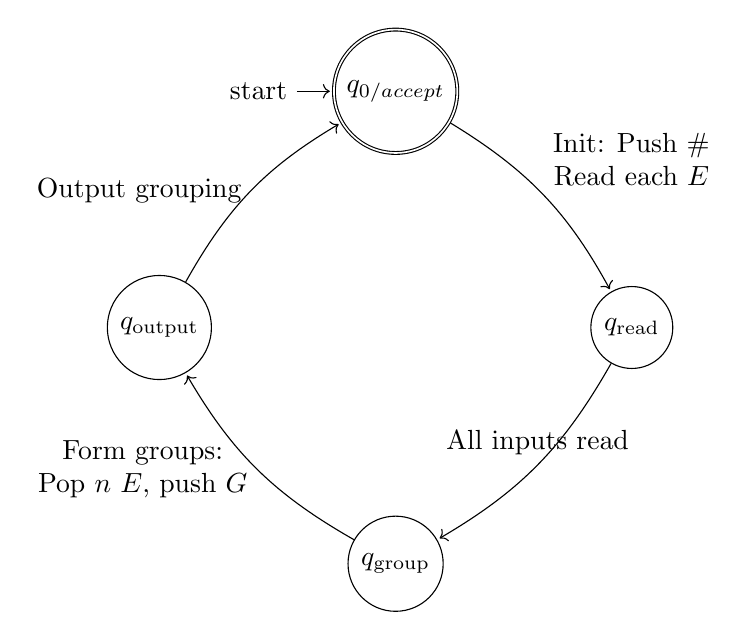
\begin{tikzpicture}[
    shorten >=1pt,
    auto,
    node distance=3cm,
    every state/.style={minimum size=1cm}
]
    % Arrange four states in a circle: 
    % q_{0/accept} at 90°, q_read at 0°, q_group at 270°, q_output at 180°
    \node[state, initial, accepting] (q0) at (90:3cm) {$q_{0/accept}$};
    \node[state] (q1) at (0:3cm) {$q_{\text{read}}$};
    \node[state] (q2) at (270:3cm) {$q_{\text{group}}$};
    \node[state] (q3) at (180:3cm) {$q_{\text{output}}$};
    
    \path[->]
        (q0) edge[bend left=15] node[above right, align=center] {Init: Push \(\#\)\\Read each \(E\)} (q1)
        (q1) edge[bend left=15] node[above, align=center] {All inputs read} (q2)
        (q2) edge[bend left=15] node[left, align=center] {Form groups:\\Pop \(n\) \(E\), push \(G\)} (q3)
        (q3) edge[bend left=15] node[left, align=center] {Output grouping} (q0);
\end{tikzpicture}
    \caption{PDA for Conversion to Groups Other than Bases}
\end{figure}
\subsubsection*{Example Execution}
\textbf{Problem:} Convert 32 items into groups of 8 in base ten.

\begin{enumerate}
    \item \textbf{Initialization:} 
    \begin{itemize}
        \item Start with the stack: \(\#\).
    \end{itemize}
    \item \textbf{Reading Total Items:}
    \begin{itemize}
        \item Read 32 elements, pushing 32 \(E\) symbols onto the stack.
    \end{itemize}
    \item \textbf{Forming Groups of 8:}
    \begin{itemize}
        \item Pop 8 \(E\) symbols and push \(G\) onto the stack.
        \item Repeat this process 4 times to form 4 groups.
    \end{itemize}
    \item \textbf{Final Stack Configuration:} \(\# \; G \; G \; G \; G\)
\end{enumerate}

\subsubsection*{Recursive Handling of Group Formation}
The PDA recursively forms groups by repeatedly popping a fixed number of elements and pushing a group identifier until all elements are grouped. This ensures the conversion of the total into groups that are not aligned with the standard base system.




\clearpage

\subsubsection*{HTML Implementation}
\lstinputlisting[style=htmlStyle, language=html]{./new_html/SMR_DIV_CGOB.html}

\printbibliography

\end{document}